%%%%%%%%%%%%%%%%%%%%%%%%%%%%%%%%%%%%%%%%%%%%%%%%%%%
%% LaTeX book template                           %%
%% Author:  Amber Jain (http://amberj.devio.us/) %%
%% License: ISC license                          %%
%%%%%%%%%%%%%%%%%%%%%%%%%%%%%%%%%%%%%%%%%%%%%%%%%%%

\documentclass[a4paper,12pt]{book}
\usepackage[T1]{fontenc}
\usepackage[utf8]{inputenc}
\usepackage[left=2cm,right=1cm,top=2cm,bottom=2cm,headheight=1cm]{geometry}
\usepackage{graphicx}
\usepackage{lmodern}
\usepackage{blindtext}


%%%%%%%%%%%%%%%%%%%%%%%%%%%%%%%%%%%%%%%%%%%%%%%%%%%%%%%%%
% Configurações para o Maxima %
%%%%%%%%%%%%%%%%%%%%%%%%%%%%%%%%%%%%%%%%%%%%%%%%%%%%%%%%%

\usepackage{graphicx}
\usepackage{color}
\usepackage{amsmath}
\usepackage{grffile}
\usepackage{ifthen}
\newsavebox{\picturebox}
\newlength{\pictureboxwidth}
\newlength{\pictureboxheight}
\newcommand{\includeimage}[1]{
    \savebox{\picturebox}{\includegraphics{#1}}
    \settoheight{\pictureboxheight}{\usebox{\picturebox}}
    \settowidth{\pictureboxwidth}{\usebox{\picturebox}}
    \ifthenelse{\lengthtest{\pictureboxwidth > .95\linewidth}}
    {
        \includegraphics[width=.95\linewidth,height=.80\textheight,keepaspectratio]{#1}
    }
    {
        \ifthenelse{\lengthtest{\pictureboxheight>.80\textheight}}
        {
            \includegraphics[width=.95\linewidth,height=.80\textheight,keepaspectratio]{#1}
            
        }
        {
            \includegraphics{#1}
        }
    }
}
\newlength{\thislabelwidth}
\DeclareMathOperator{\abs}{abs}

\definecolor{labelcolor}{RGB}{100,0,0}



%%%%%%%%%%%%%%%%%%%%%%%%%%%%%%%%%%%%%%%%%%%%%%%%%%%%%%%%%
% Source: http://en.wikibooks.org/wiki/LaTeX/Hyperlinks %
%%%%%%%%%%%%%%%%%%%%%%%%%%%%%%%%%%%%%%%%%%%%%%%%%%%%%%%%%
\usepackage{hyperref}
%\usepackage{graphicx}
\usepackage[portuguese]{babel}

%%%%%%%%%%%%%%%%%%%%%%%%%%%%%%%%%%%%%%%%%%%%%%%%%%%%%%%%%%%%%%%%%%%%%%%%%%%%%%%%
% 'dedication' environment: To add a dedication paragraph at the start of book %
% Source: http://www.tug.org/pipermail/texhax/2010-June/015184.html            %
%%%%%%%%%%%%%%%%%%%%%%%%%%%%%%%%%%%%%%%%%%%%%%%%%%%%%%%%%%%%%%%%%%%%%%%%%%%%%%%%
\newenvironment{dedication}
{
   \cleardoublepage
   \thispagestyle{empty}
   \vspace*{\stretch{1}}
   \hfill\begin{minipage}[t]{0.66\textwidth}
   \raggedright
}
{
   \end{minipage}
   \vspace*{\stretch{3}}
   \clearpage
}

%%%%%%%%%%%%%%%%%%%%%%%%%%%%%%%%%%%%%%%%%%%%%%%%
% Chapter quote at the start of chapter        %
% Source: http://tex.stackexchange.com/a/53380 %
%%%%%%%%%%%%%%%%%%%%%%%%%%%%%%%%%%%%%%%%%%%%%%%%
\makeatletter
\renewcommand{\@chapapp}{}% Not necessary...
\newenvironment{chapquote}[2][2em]
  {\setlength{\@tempdima}{#1}%
   \def\chapquote@author{#2}%
   \parshape 1 \@tempdima \dimexpr\textwidth-2\@tempdima\relax%
   \itshape}
  {\par\normalfont\hfill--\ \chapquote@author\hspace*{\@tempdima}\par\bigskip}
\makeatother


%%%%%%%%%%%%%%%%%%%%%%%%%%%%%%%%%%%%%%%%%%%%%%%%%%%
% First page of book which contains 'stuff' like: %
%  - Book title, subtitle                         %
%  - Book author name                             %
%%%%%%%%%%%%%%%%%%%%%%%%%%%%%%%%%%%%%%%%%%%%%%%%%%%

% Book's title and subtitle
\title{\Huge \textbf{\MakeUppercase{Simulações de Ondulatória com Uso do Maxima}} \footnote{This is a footnote.} \\  }
% Author
\author{\textsc{Elielzer Nuayed}\thanks{\url{www.example.com}}}


\begin{document}

\frontmatter
\maketitle

%%%%%%%%%%%%%%%%%%%%%%%%%%%%%%%%%%%%%%%%%%%%%%%%%%%%%%%%%%%%%%%
% Add a dedication paragraph to dedicate your book to someone %
%%%%%%%%%%%%%%%%%%%%%%%%%%%%%%%%%%%%%%%%%%%%%%%%%%%%%%%%%%%%%%%
\begin{dedication}
Dedicated to Calvin and Hobbes.
\end{dedication}

%%%%%%%%%%%%%%%%%%%%%%%%%%%%%%%%%%%%%%%%%%%%%%%%%%%%%%%%%%%%%%%%%%%%%%%%
% Auto-generated table of contents, list of figures and list of tables %
%%%%%%%%%%%%%%%%%%%%%%%%%%%%%%%%%%%%%%%%%%%%%%%%%%%%%%%%%%%%%%%%%%%%%%%%
{\tableofcontents}
{\listoffigures}
{\listoftables}

\mainmatter

%%%%%%%%%%%
% Preface %
%%%%%%%%%%%
\chapter*{Preface}
Este livro foi concebido a partir de um \emph{insight} pessoal após eu ler um anúncio sobre uso do \emph{Maxima} no ensino da Física. Então veio-me a ideia de escrever algo nesse sentido.
Escolhi sobre ondulatória. O Maxima é introduzido no contexto como ambiente de apoio no momento que seja necessário simular as proposições. Dentre as proposições abordaremos situações clássicas, pois o objetivo é justamente apresentar o cartel de
ferramentas desse software adequadas para transcrever a linguagem da física para representar as situações problema.



%%%%%%%%%%%%%%%%
% NEW CHAPTER! %
%%%%%%%%%%%%%%%%
\chapter{INTRODUÇÃO}

\begin{chapquote}{Author's name, \textit{Source of this quote}}
``This is a quote and I don't know who said this.''
\end{chapquote}

\section{Um Pouco Sobre Ondas}
Há várias situações no dia a dia nas quais as coisas acontecem repentinamente, ou inesperadamente, vindo, depois a cessar seus efeitos, ou, em outros casos, repercutem mais além. É comum nos referirmos a isso com a expressão: "isso é apenas uma onda, logo passará". Isso, claro, devido a que tais situações são transitórias, exemplos: pandemias, endemias, o preço de commodities, tsunamis, terremotos, até notícias ou eventos cotidianos. Algumas vezes tais situações apresentam comportamento oscilante, como na superfície de um líquido em uma piscina, ou mesmo em fontes naturais de água, como em rios, mares e oceanos durante a passagem de uma embarcação.

É importante notar que existem características diferentes em tais situações. Alguns simplesmente oscilam ou vibram e em outros casos, além de oscilar ou vibrar, essa condição é posteriormente transmitida para outros locais do ambiente onde tais situações ocorrem. Neste segundo caso, diz-se que há uma propagação do fenômeno. De tal forma que, oscilação, onda, propagação são termos correlacionados.

Etimologicamente, a palavra onda teria a ver com o significado de algo que flutua na água. As descobertas e desenvolvimentos neste tema em seus primórdios derivaram do estudo dos sons musicais. Diz-se que o estudo moderno de ondas e acústica se originou com \emph{Galileu Galilei}.

A figura \ref{fig:mapa.ondas} apresenta a evolução, numa perspectiva histórica, do conhecimento científico desta temática, através da contribuição de vários investigadores.

\begin{figure}[htbp!]
    \centering
    \caption{Representação da evolução do conhecimento sobre ondas.}
        \label{fig:mapa.ondas}
    %\begin{Center}
    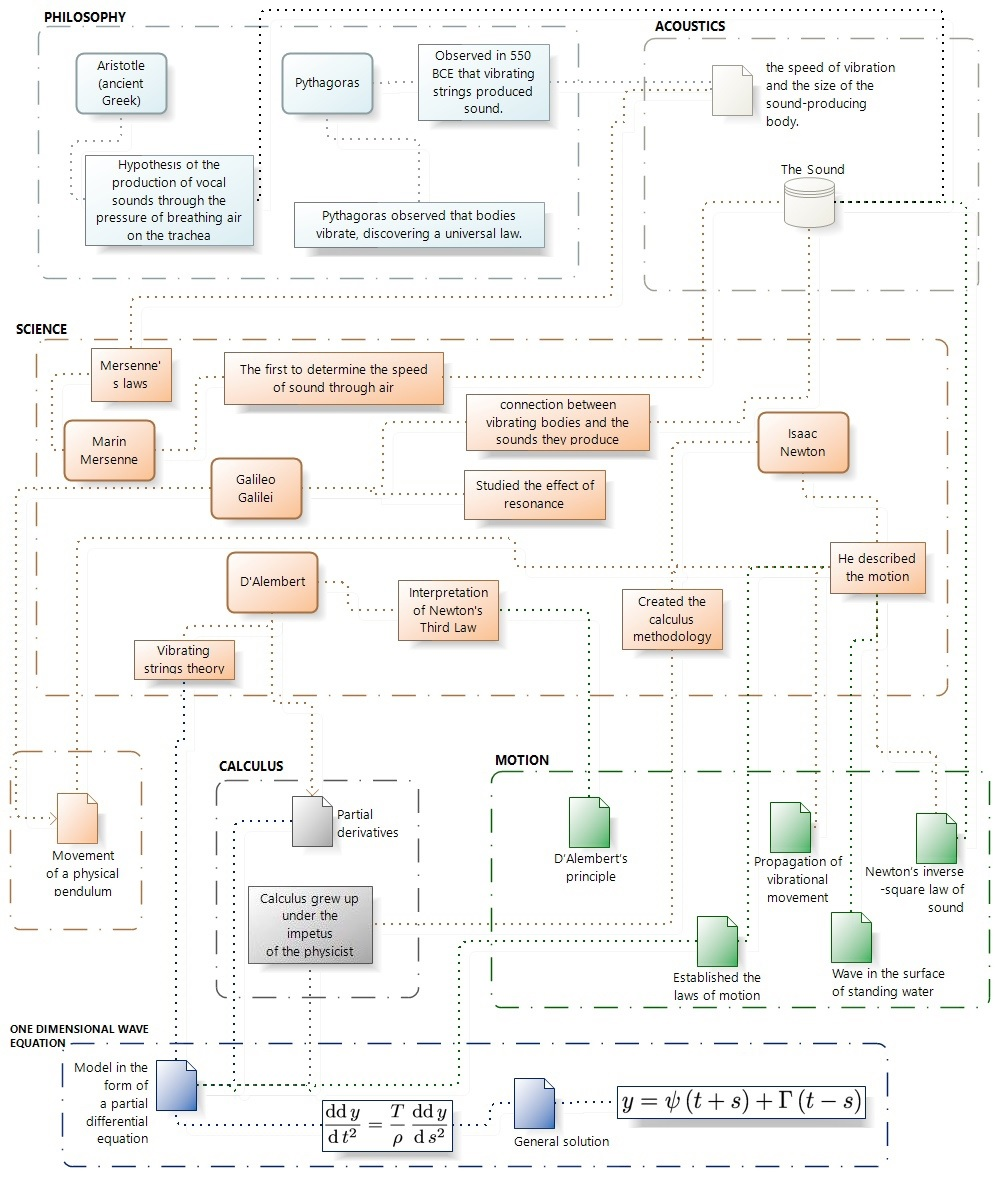
\includegraphics[width=0.95\textwidth,height=0.95\textheight]{sounds.jpg}
	%\end{Center}
\end{figure}

\newpage
\section{Sobre o Maxima}
De acordo com descrição no site fabricante, o Maxima é um programa de computador do tipo multiplataforma, ou seja, ele está preparado para trabalhar (compilar) sob diversos sistemas operacionais ou plataformas computacionais.
Ainda de acordo com esse site o Maxima é uma versão evoluída de software especialista Macsyma. Os sistemas especialistas foram criados com a finalidade de reproduzir o raciocínio ou expertise de um  profissional de alguma área de conhecimento específica.

Assm,o Maxima é um sistema especialista para a manipulação de expressões matemáticas, tanto na forma simbólica como na forma numérica, incluindo:
\begin{itemize}
    \item diferenciação,
    \item integração,
    \item séries de Taylor,
    \item transformadas de Laplace,
    \item equações diferenciais ordinárias,
    \item sistemas de equações lineares,
    \item polinômios,
    \item conjuntos,
    \item listas,
    \item vetores,
    \item matrizes e
    \item tensores.
\end{itemize}

\noindent O que caracteriza a matemática simbólica é de não estar atrelada a um determinado idioma, por exemplo a expressão algébrica: \(x+2=7\), tem o mesmo significado em qualquer idioma. Portanto o Maxima é um sistema algébrico computacional para auxílio no cálculo e manipulação da  matemática simbólica visado simplificar o esforço de trabalho do estudante ou profissional (professor ou pesquisador).

O Maxima produz também resultados numéricos de alta precisão usando frações exatas, inteiros de precisão arbitrária e números de ponto flutuante de precisão variável. O Maxima pode plotar funções e dados em duas e três dimensões.

%%%%%%%%%%%%%%%%%%%%%%%%%%%%%%%%%%%%%%%%%%%%%%%%%%%%%%%
% Sample table                                        %
% Source: www1.maths.leeds.ac.uk/latex/TableHelp1.pdf %
%%%%%%%%%%%%%%%%%%%%%%%%%%%%%%%%%%%%%%%%%%%%%%%%%%%%%%%
\begin{table}[ht]
\caption{Sample table} % title of Table
\centering % used for centering table
\begin{tabular}{c c c c}
% centered columns (4 columns)
\hline\hline %inserts double horizontal lines
S. No. & Column\#1 & Column\#2 & Column\#3 \\ [0.5ex]
% inserts table
%heading
\hline % inserts single horizontal line
1 & 50 & 837 & 970 \\
2 & 47 & 877 & 230 \\
3 & 31 & 25 & 415 \\
4 & 35 & 144 & 2356 \\
5 & 45 & 300 & 556 \\ [1ex] % [1ex] adds vertical space
\hline %inserts single line
\end{tabular}
\label{table:nonlin} % is used to refer this table in the text
\end{table}
\section{Como instalar o Maxima}
Instalar um software é uma tarefa que a maioria de usuários de PC já fizeram alguma vez, e instalar o Maxima é uma tarefa que não haverá muita dificuldade. O primeiro passo é obter o arquivo instalador. Uma opção é fazer o processo de \emph{download} do endereço da internet ou URL (sugestão do autor): maxima.sourceforge.io/windows-install.html (\ref{fig:site-maxima}). 
\begin{figure}[htbp!]
    \centering
    \caption{Entrando com a URL, para buscar a página do Maxima no \emph{Google}.}
        \label{fig:site-maxima}
    %\begin{Center}
    
\includegraphics[]{site-maxima.jpg}
	%\end{Center}
\end{figure}

\noindent A página na figura \ref{fig:pagina-maxima} contém um passo a passo, que é recomendável que seja lido. Entretando, por ora seguiremos mais focados no processo operacional de instalação em si. 
Assim, localize o link, nessa página com o texto: \href{sourceforge.net/projects/maxima/files/Maxima-Windows/5.46.0-Windows/}{5.46.0-Windows}, como mostrado nessa imagem.

\begin{figure}[htbp!]
    \centering
    \caption{Página encontrada do Maxima no navegador da Internet.}
        \label{fig:pagina-maxima}
    %\begin{Center}
    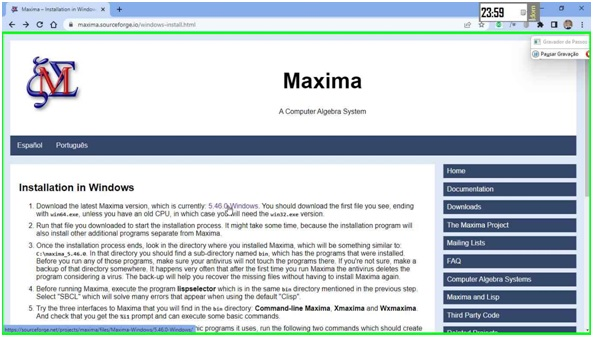
\includegraphics[]{pagina-maxima.jpg}
	%\end{Center}	
\end{figure}
\newpage
\noindent	Como forma de gerenciar o processo de instalação são apresentadas a seguir as janelas que interagem nas diversa etapas dessa instalação.
	\begin{figure}[htbp!]
    \centering
    \caption{Janela que apresenta o início do processo de instalação.}
        \label{fig:maxima-ist-1}
    %\begin{Center}
    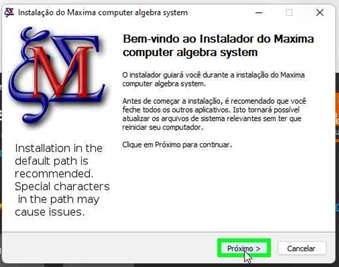
\includegraphics[]{maxima-ist-1.jpg}
	%\end{Center}
\end{figure}


	\begin{figure}[htbp!]
    \centering
    \caption{Janela que apresenta os termos de uso.}
        \label{fig:maxima-ist-2}
    %\begin{Center}
    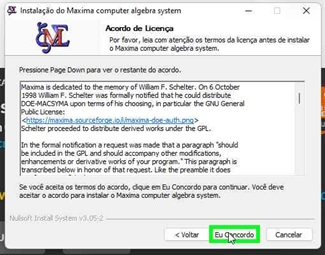
\includegraphics[]{maxima-ist-2.jpg}
	%\end{Center}
\end{figure}

	\begin{figure}[htbp!]
    \centering
    \caption{Janela que apresenta o diretório local para instalação de arquivos.}
        \label{fig:maxima-ist-3}
    %\begin{Center}
    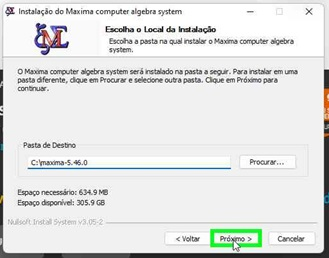
\includegraphics[]{maxima-ist-3.jpg}
	%\end{Center}
\end{figure}

	\begin{figure}[htbp!]
    \centering
    \caption{Janela de configuração de atalhos.}
        \label{fig:maxima-ist-4}
    %\begin{Center}
    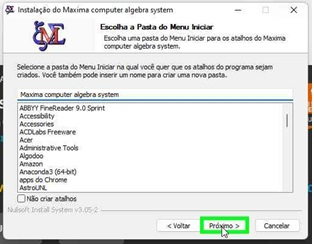
\includegraphics[]{maxima-ist-4.jpg}
	%\end{Center}
\end{figure}

	\begin{figure}[htbp!]
    \centering
    \caption{Janela de configuração do escopo de funções do programa.}
        \label{fig:maxima-ist-5}
    %\begin{Center}
    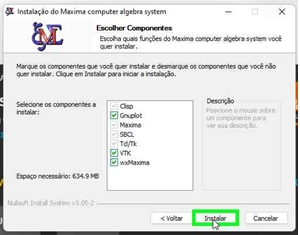
\includegraphics[]{maxima-ist-5.jpg}
	%\end{Center}
\end{figure}

	\begin{figure}[htbp!]
    \centering
    \caption{Janela de status do processo de instalação.}
        \label{fig:maxima-ist-6}
    %\begin{Center}
    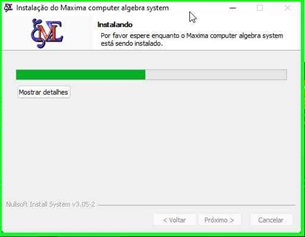
\includegraphics[]{maxima-ist-6.jpg}
	%\end{Center}
\end{figure}

	\begin{figure}[htbp!]
    \centering
    \caption{Janela de confirmação da instalação.}
        \label{fig:maxima-ist-7}
    %\begin{Center}
    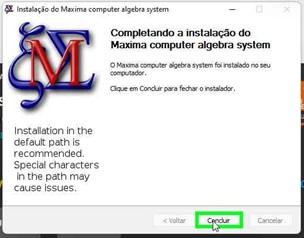
\includegraphics[]{maxima-ist-7.jpg}
	%\end{Center}
\end{figure}

	\begin{figure}[htbp!]
    \centering
    \caption{Aspecto do comando de menu na janela inicial do Windows.}
        \label{fig:menu-windows}
    %\begin{Center}
    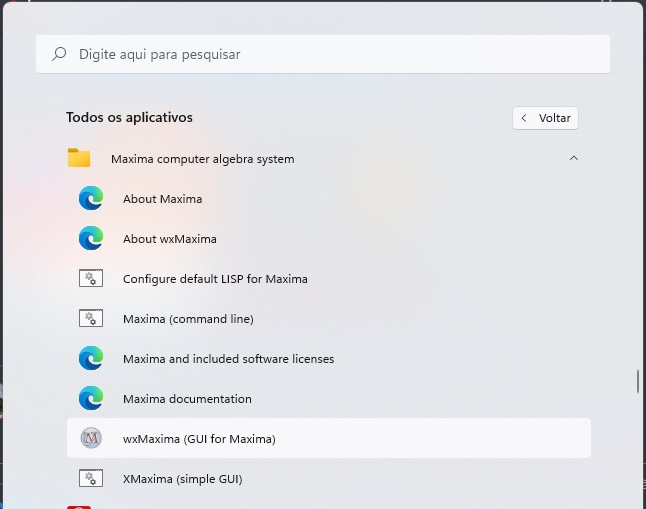
\includegraphics[scale=0.7]{menu-windows.jpg}
	%\end{Center}
\end{figure}
\newpage
\section{Conhecendo a \emph{interface} do aplicativo}
A janela do aplicativo Maxima é idêntica a um editor de texto. Ao abrir a janela, esta já fornece de imediato um prompt para a entrada de comandos de programação, ou textos descritivos. 
	\begin{figure}[htbp!]
    \centering
    \caption{Aspecto da janela do aplicativo Maxima.}
        \label{fig:tela-inicial}
    %\begin{Center}
    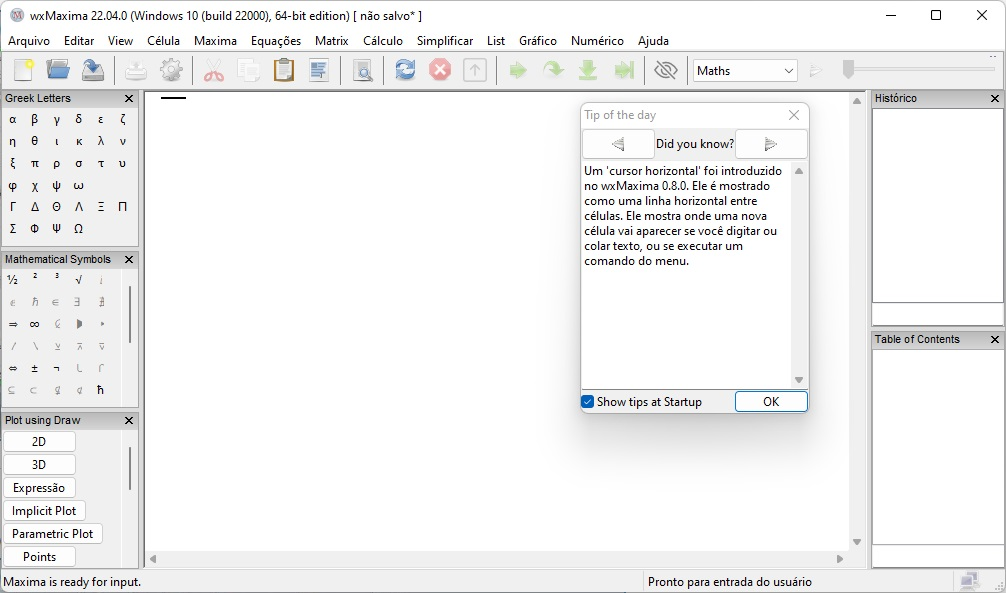
\includegraphics[scale=0.6]{tela-inicial.jpg}
	%\end{Center}
\end{figure}


\noindent A figura \ref{fig:selecao-tipos} mostra como escolhar as opções de tipo de entrada no prompt para o caso de texto
	\begin{figure}[htbp!]
    \centering
    \caption{Pré-seleção para inserir texto no prompt.}
        \label{fig:selecao-tipos}
    %\begin{Center}
    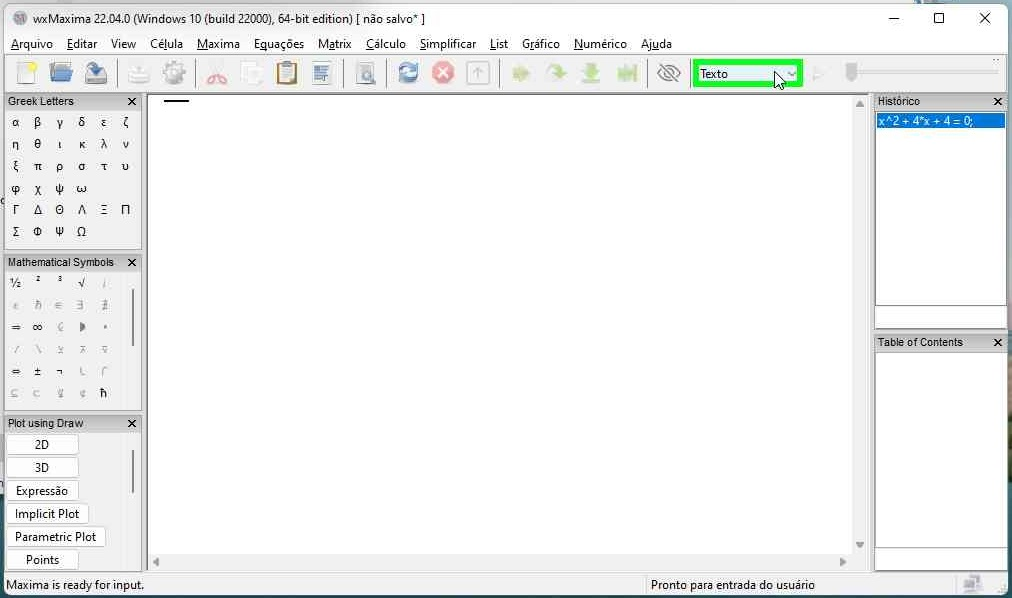
\includegraphics[scale=0.6]{selecao-tipos.jpg}
	%\end{Center}
\end{figure}

\noindent A figura \ref{fig:selecao-texto} mostra como escolher as opções de tipo de entrada no prompt para o caso de texto. Já a figura \ref{fig:selecao-math} mostra como escolher as opções de tipo de entrada no prompt para o caso de texto
	\begin{figure}[htbp!]
    \centering
    \caption{Pré-seleção para inserir texto no prompt.}
        \label{fig:selecao-texto}
    %\begin{Center}
    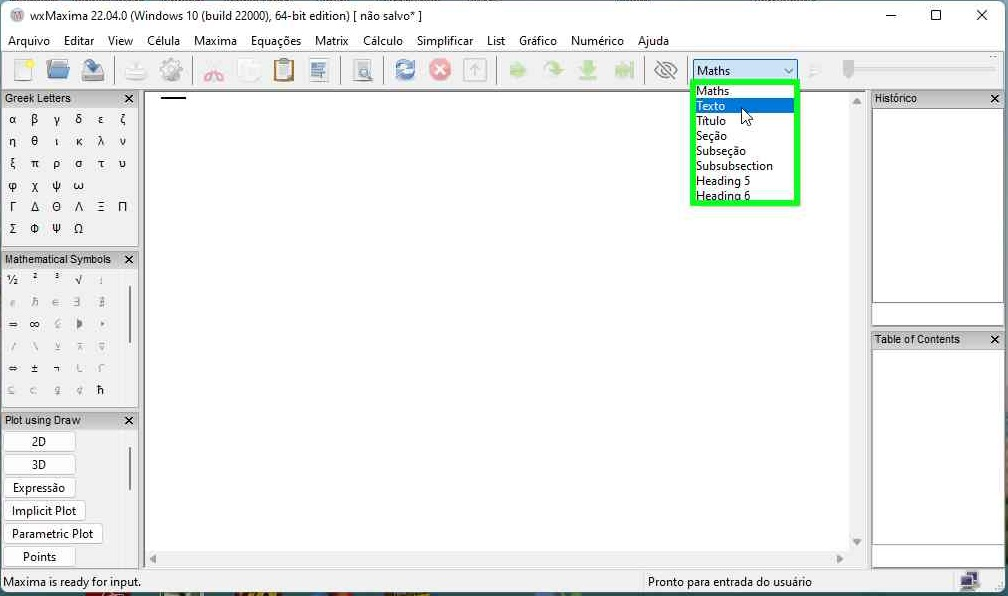
\includegraphics[scale=0.6]{selecao-texto.jpg}
	%\end{Center}
\end{figure}


	\begin{figure}[htbp!]
    \centering
    \caption{Pré-seleção para inserir expressão algébrica no prompt.}
        \label{fig:selecao-math}
    %\begin{Center}
    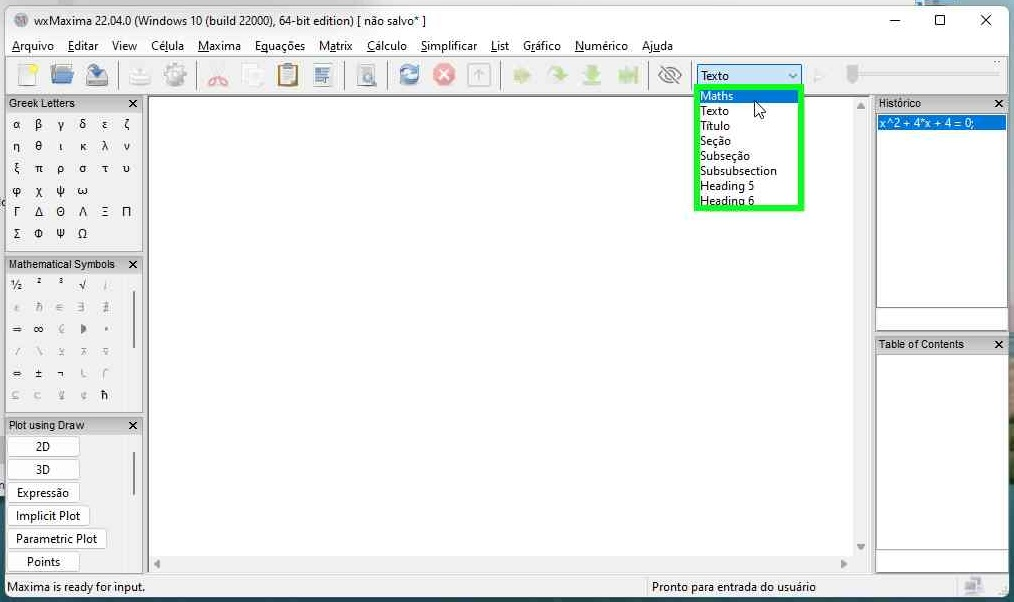
\includegraphics[scale=0.6]{selecao-math.jpg}
	%\end{Center}
\end{figure}
Até agora nos ativemos a apresentar generalidades que subsidiarão o leitor durante sua jornada no aprendizado ou mesmo na utilização das técnica aqui apresntadas de simulação no Maxima. Assunto que será objeto dos próximos capítulos.

\chapter{Trabalhando com o Maxima}

\noindent
%%%%%%%%
%% INPUT:
\begin{minipage}[t]{4.000000em}\color{red}\bfseries
(\% i1)	
\end{minipage}
\begin{minipage}[t]{\textwidth}\color{blue}
pitg:c\^\ 2+b\^\ 2=a\^\ 2;
\end{minipage}
%%%% OUTPUT:
\[\displaystyle \tag{\% o1} 
{{c}^{2}}+{{b}^{2}}={{a}^{2}}\mbox{}
\]
%%%%%%%%%%%%%%%%

\end{document}
